\clearpage
\section{Raw results from the first U.S. complementary survey}
% TODO! socio-demos, vote, interest politics, left_right, govt_involvement, donation_charities, bias, feedback

% \begin{figure}[h!]
%     \caption{label}\label{fig:vars}
%     \makebox[\textwidth][c]{\includegraphics[width=\textwidth]{../figures/US1/vars.pdf}} 
% \end{figure}

\begin{figure}[h!]
    \caption{Correct answers to comprehension questions.}\label{fig:understood_each}
    \makebox[\textwidth][c]{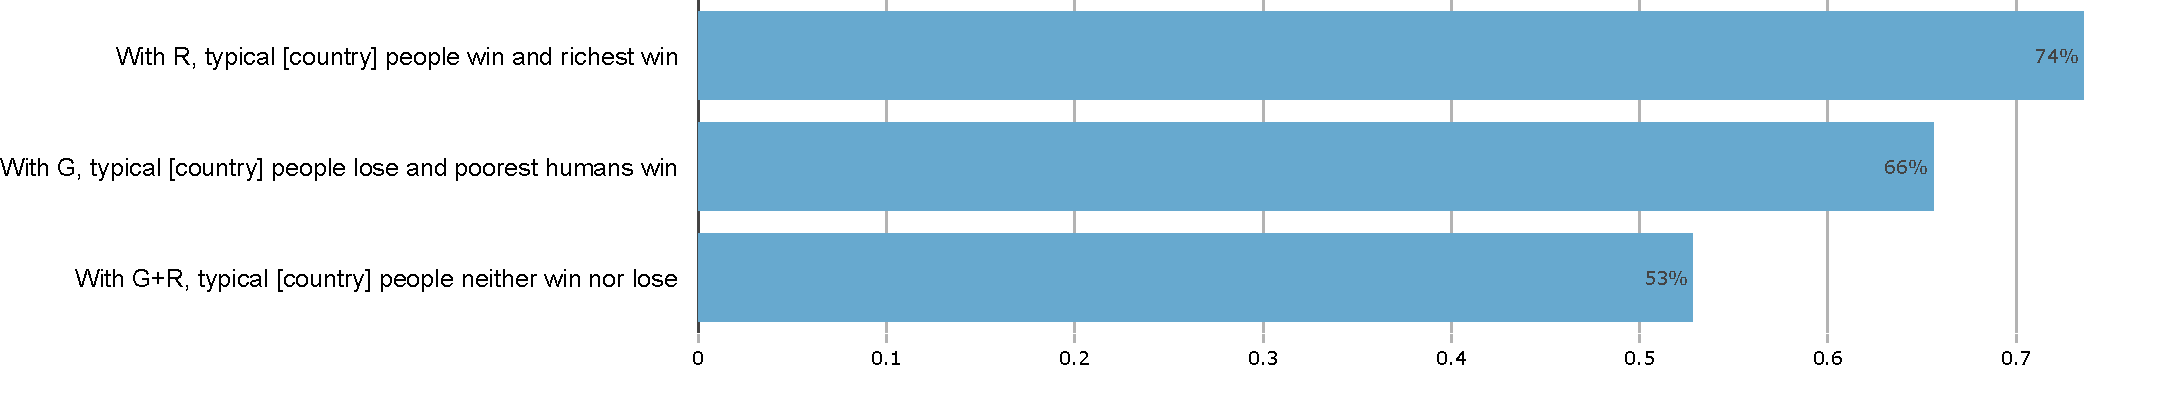
\includegraphics[width=\textwidth]{../figures/US1/understood_each.pdf}} 
\end{figure}

\begin{figure}[h!]
    \caption{Number of correct answers to comprehension questions.}\label{fig:understood_score}
    \makebox[\textwidth][c]{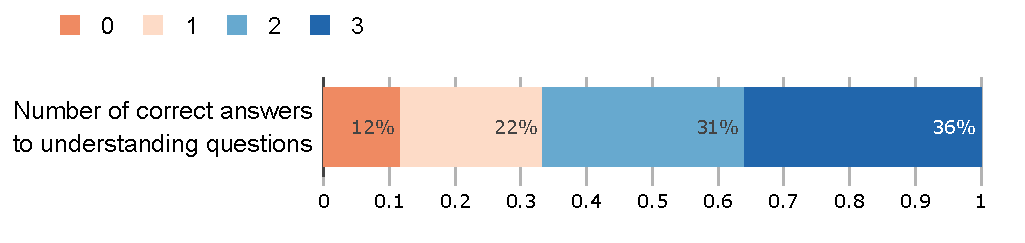
\includegraphics[width=\textwidth]{../figures/US1/understood_score.pdf}} 
\end{figure}

\begin{figure}[h!]
    \caption{Support for the GCS, NC and the combination of GCS, NR and C.}\label{fig:support_binary}
    \makebox[\textwidth][c]{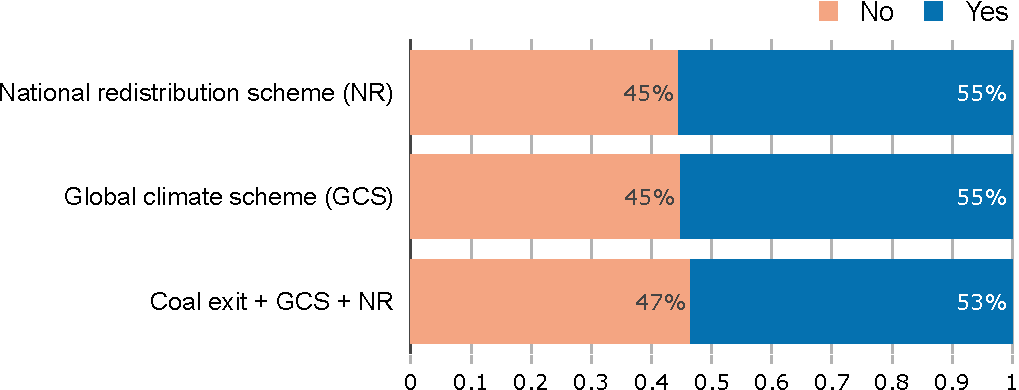
\includegraphics[width=\textwidth]{../figures/US1/support_binary.pdf}} 
\end{figure}

\begin{figure}[h!]
    \caption{Beliefs regarding the support for the GCS and NR.}\label{fig:belief}
    \makebox[\textwidth][c]{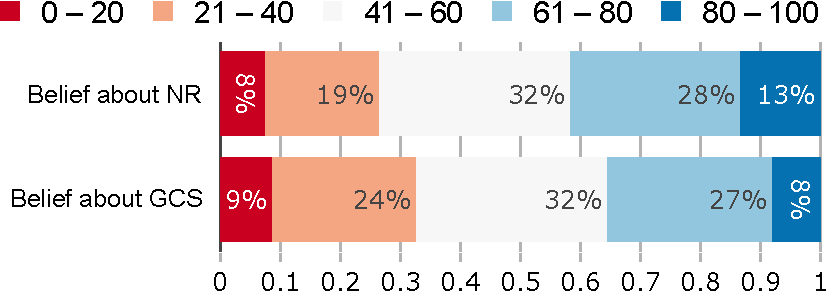
\includegraphics[width=\textwidth]{../figures/US1/belief.pdf}} 
\end{figure}

\begin{figure}[h!]
    \caption{List experiment.}\label{fig:list_exp}
    \makebox[\textwidth][c]{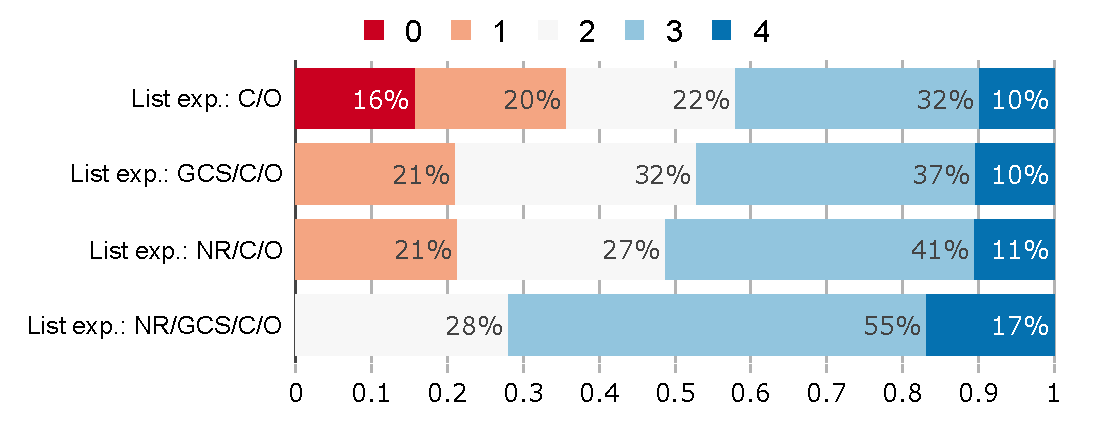
\includegraphics[width=\textwidth]{../figures/US1/list_exp.pdf}} 
\end{figure}

\begin{figure}[h!]
    \caption{Conjoint analyses.}\label{fig:conjoint}
    \makebox[\textwidth][c]{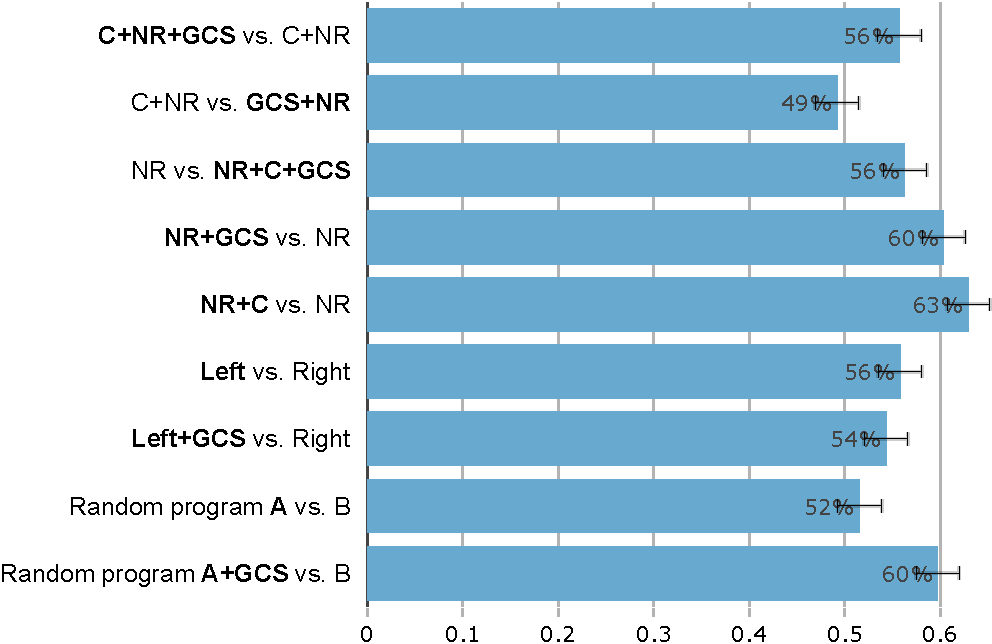
\includegraphics[width=\textwidth]{../figures/US1/conjoint.pdf}} 
\end{figure}

\begin{figure}[h!] % already in text
    \caption{[Asked only to non-Republicans] Conjoint analysis n°4: random programs at the Democratic primary.}\label{fig:ca_r}
    \makebox[\textwidth][c]{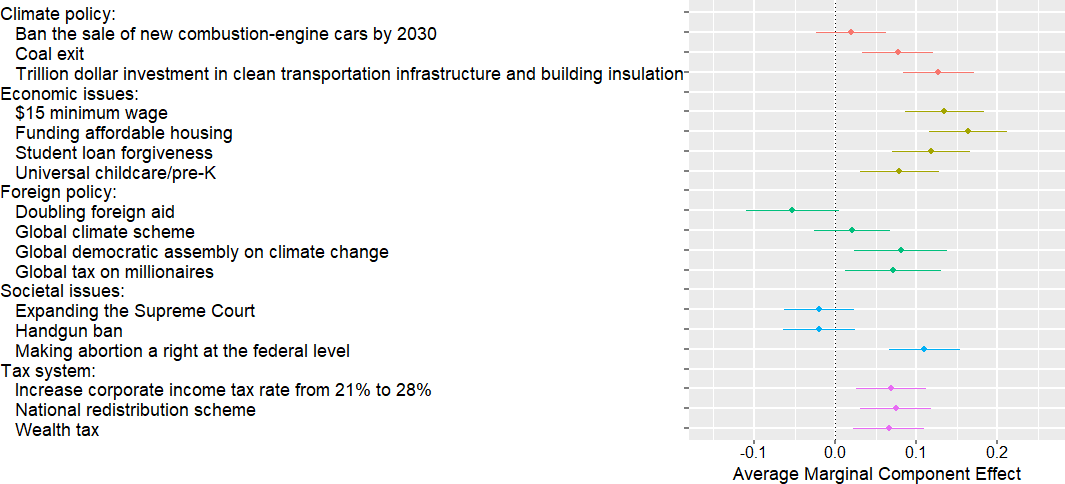
\includegraphics[width=\textwidth]{../figures/US1/ca_r.png}} 
\end{figure}

\begin{figure}[h!]
    \caption{Donation in case of lottery win.}\label{fig:variables_donation}
    \makebox[\textwidth][c]{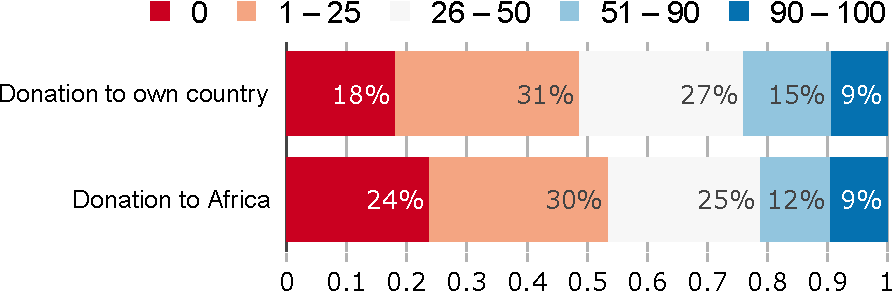
\includegraphics[width=\textwidth]{../figures/US1/variables_donation.pdf}} 
\end{figure}

\begin{figure}[h!]
    \caption{Willingness to sign real-stake petition for the GCS or NR.}\label{fig:variables_petition}
    \makebox[\textwidth][c]{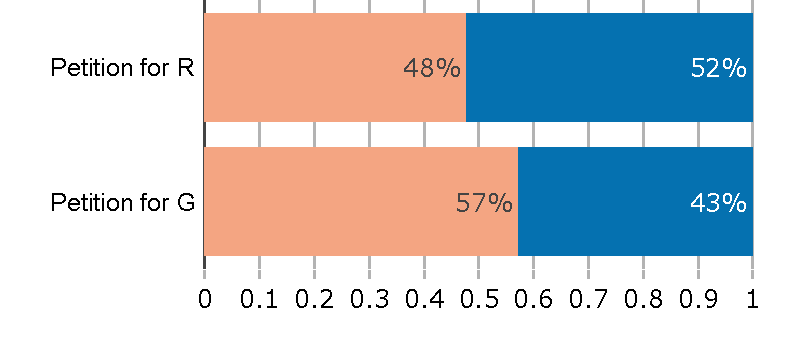
\includegraphics[width=.7\textwidth]{../figures/US1/variables_petition.pdf}} 
\end{figure}

\begin{figure}[h!] % already in text
    \caption{Support for various global policies.}\label{fig:support_likert}
    \makebox[\textwidth][c]{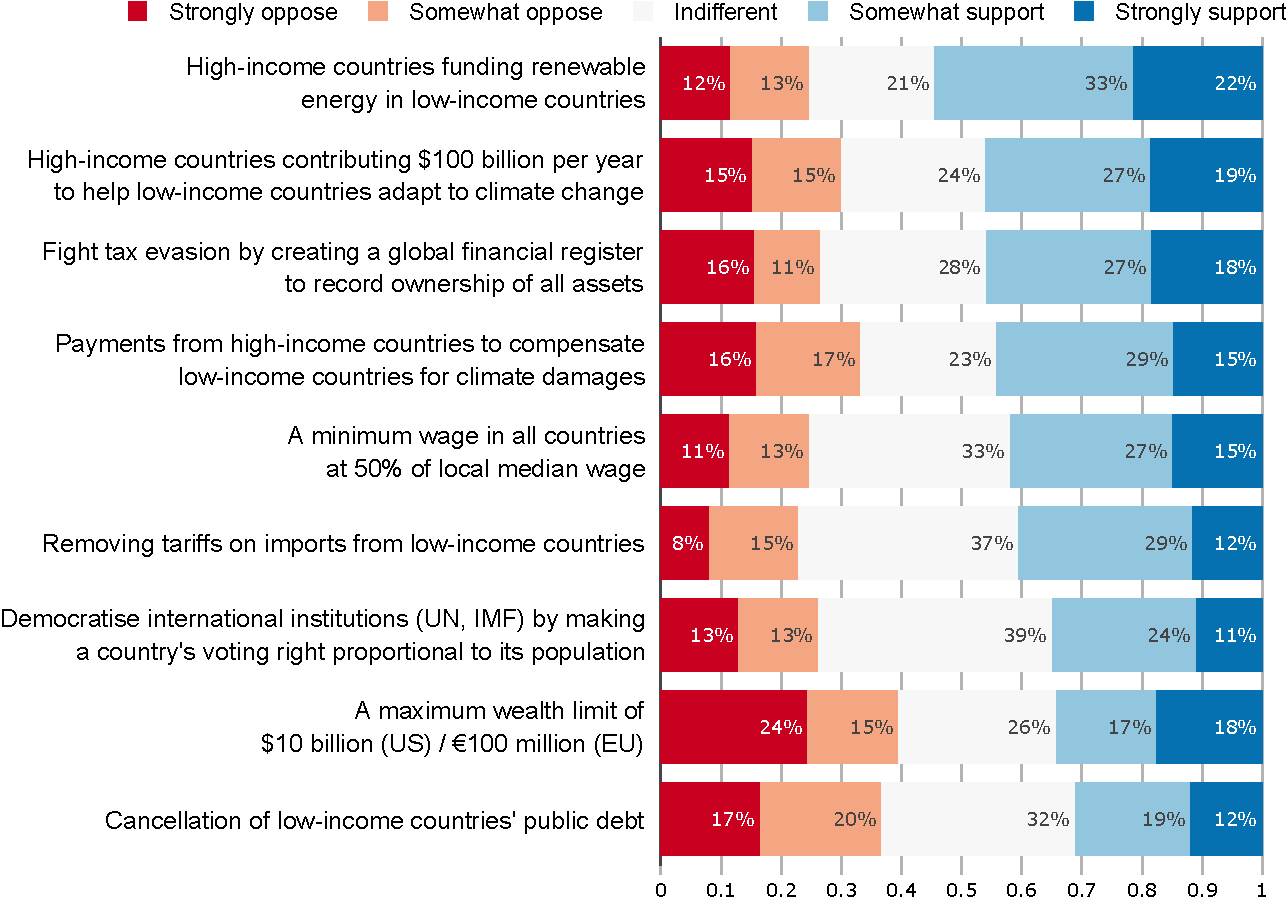
\includegraphics[width=\textwidth]{../figures/US1/support_likert.pdf}} 
\end{figure}

% \begin{figure}[h!]
%     \caption{label}\label{fig:climate_policies}
%     \makebox[\textwidth][c]{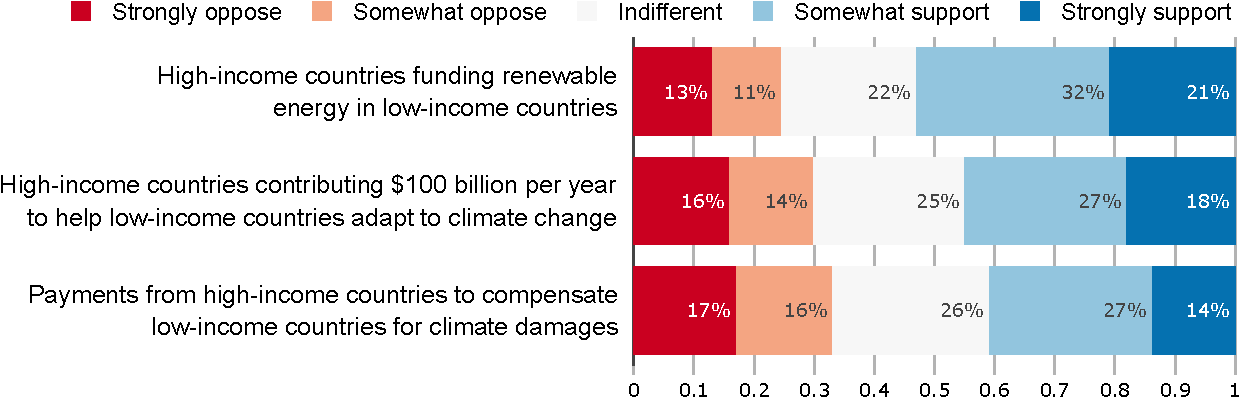
\includegraphics[width=\textwidth]{../figures/US1/climate_policies.pdf}} 
% \end{figure}

% \begin{figure}[h!]
%     \caption{label}\label{fig:global_policies}
%     \makebox[\textwidth][c]{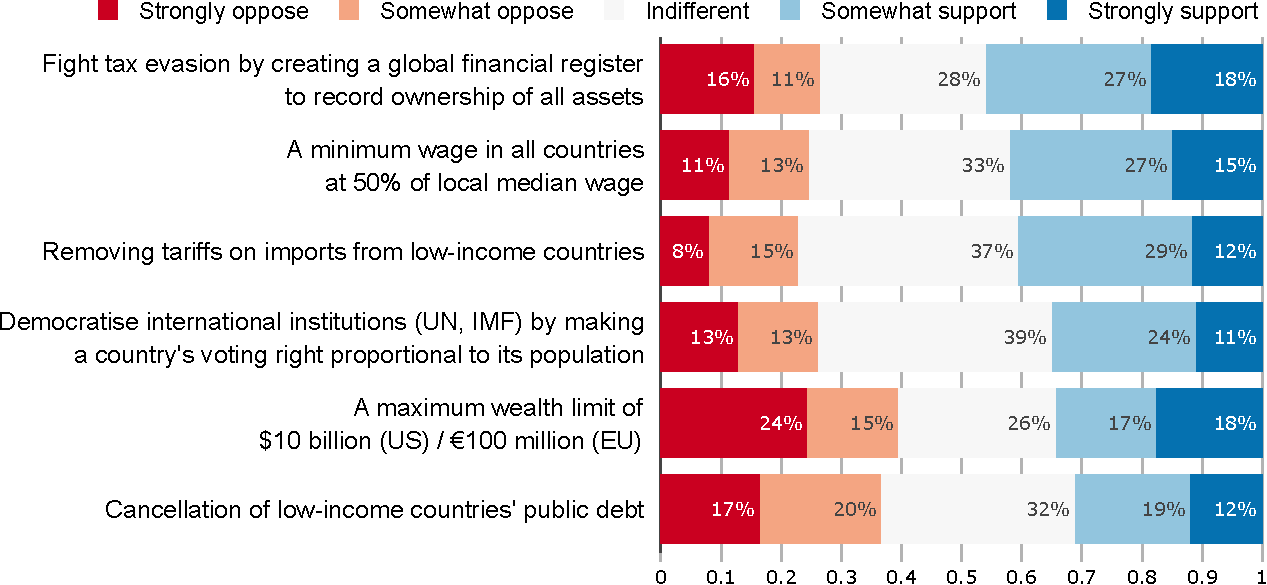
\includegraphics[width=\textwidth]{../figures/US1/global_policies.pdf}} 
% \end{figure}

\begin{figure}[h!]
    \caption{Attitudes regarding the evolution of U.S. foreign aid.}\label{fig:foreign_aid_raise_support}
    \makebox[\textwidth][c]{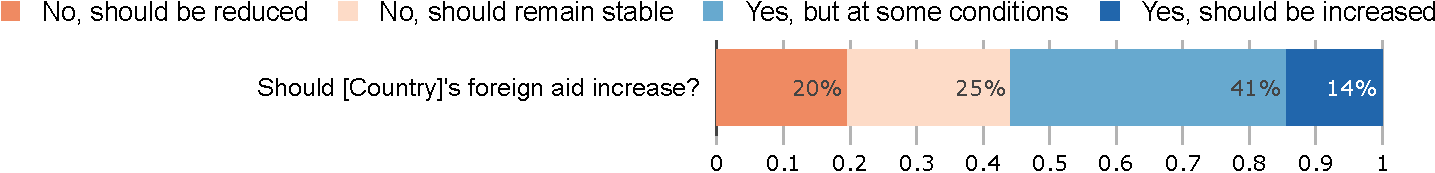
\includegraphics[width=\textwidth]{../figures/US1/foreign_aid_raise_support.pdf}} 
\end{figure}

\begin{figure}[h!]
    \caption{[Asked to those who wish an increase of foreign aid at some conditions.] Conditions at which foreign aid should be increased.}\label{fig:foreign_aid_condition}
    \makebox[\textwidth][c]{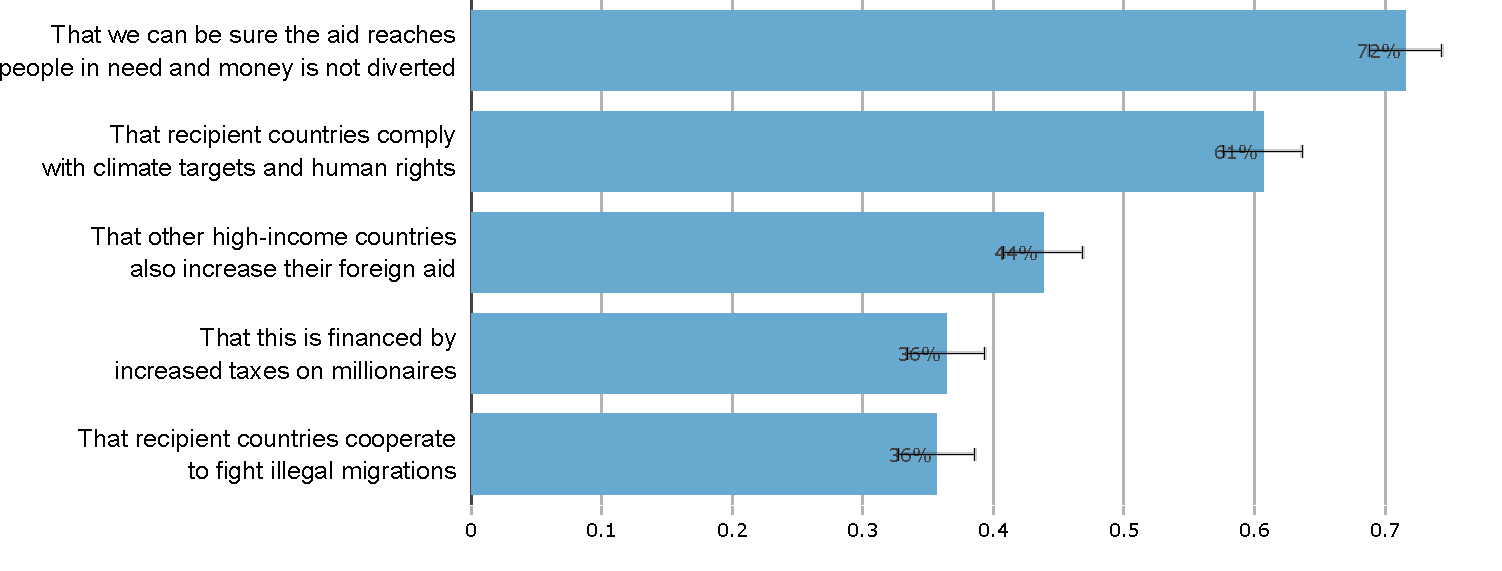
\includegraphics[width=\textwidth]{../figures/US1/foreign_aid_condition.pdf}} 
\end{figure}

\begin{figure}[h!]
    \caption{[Asked to those who wish a decrease or stability of foreign aid.] Reasons why foreign aid should not be increased.}\label{fig:foreign_aid_no}
    \makebox[\textwidth][c]{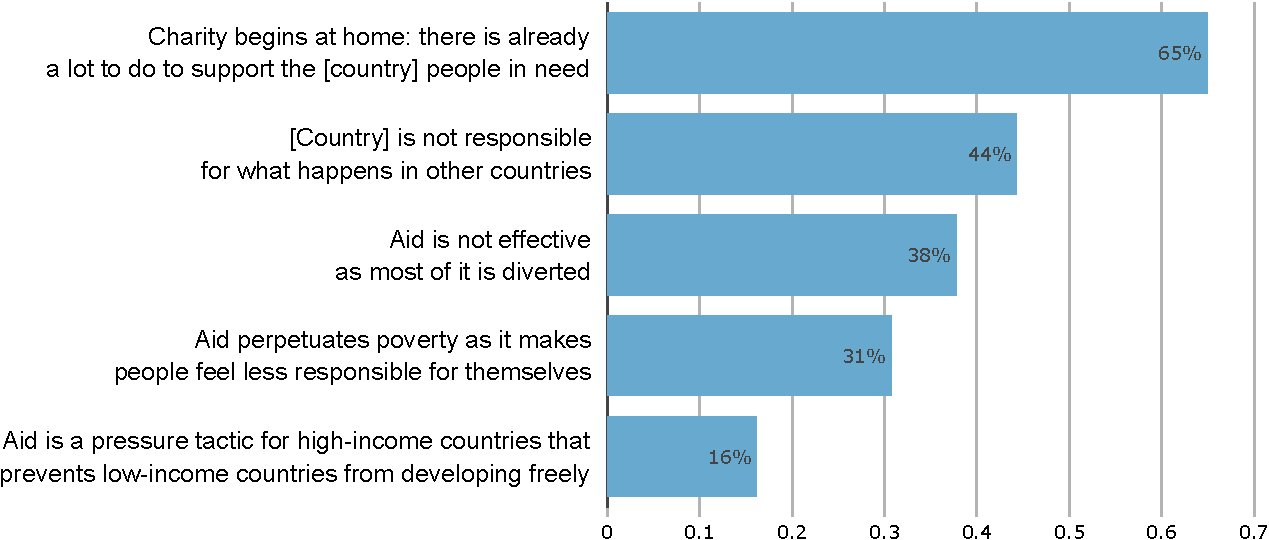
\includegraphics[width=\textwidth]{../figures/US1/foreign_aid_no.pdf}} 
\end{figure}

\begin{figure}[h!]
    \caption{Preferred approach of U.S. diplomats at international climate negotiations.}\label{fig:negotiation}
    \makebox[\textwidth][c]{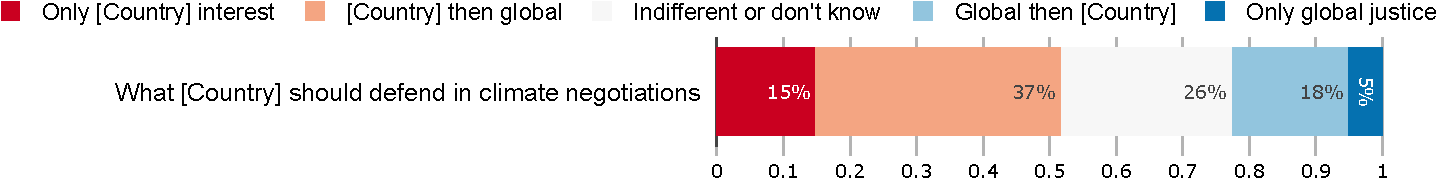
\includegraphics[width=\textwidth]{../figures/US1/negotiation.pdf}} 
\end{figure}

% \begin{figure}[h!]
%     \caption{label}\label{fig:vote}
%     \makebox[\textwidth][c]{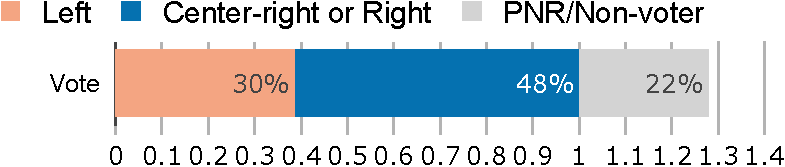
\includegraphics[width=\textwidth]{../figures/US1/vote.pdf}} 
% \end{figure}

\begin{figure}[h!]
    \caption{Extent to which selected issues are viewed as important problems.}\label{fig:problem}
    \makebox[\textwidth][c]{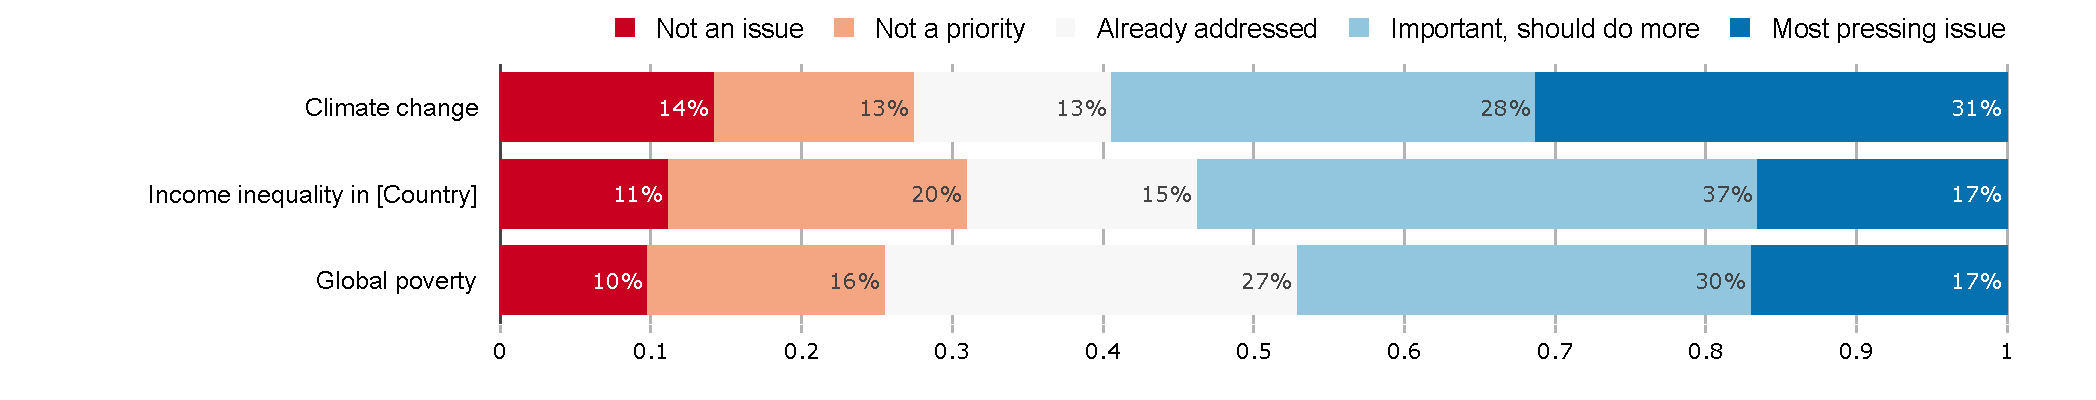
\includegraphics[width=\textwidth]{../figures/US1/problem.pdf}} 
\end{figure}

\begin{figure}[h!]
    \caption{Group defended when voting.}\label{fig:group_defended_agg}
    \makebox[\textwidth][c]{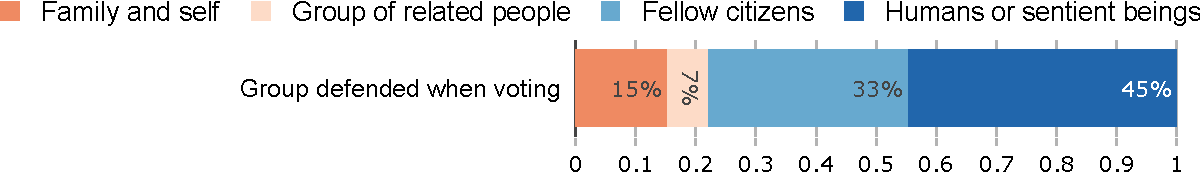
\includegraphics[width=\textwidth]{../figures/US1/group_defended_agg.pdf}} 
\end{figure}

% \begin{figure}[h!]
%     \caption{label}\label{fig:group_defended}
%     \makebox[\textwidth][c]{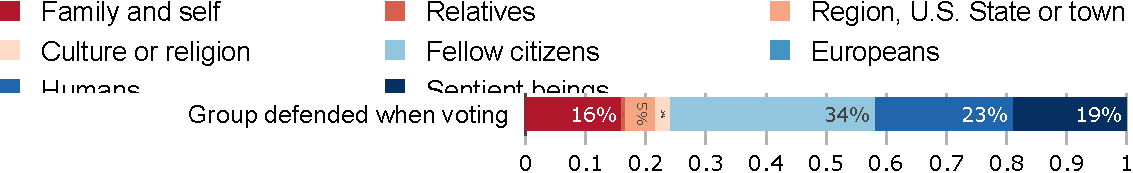
\includegraphics[width=\textwidth]{../figures/US1/group_defended.pdf}} 
% \end{figure}

\begin{figure}[h!] % already in text
    \caption{Prioritization of policies.}\label{fig:points_us}
    \makebox[\textwidth][c]{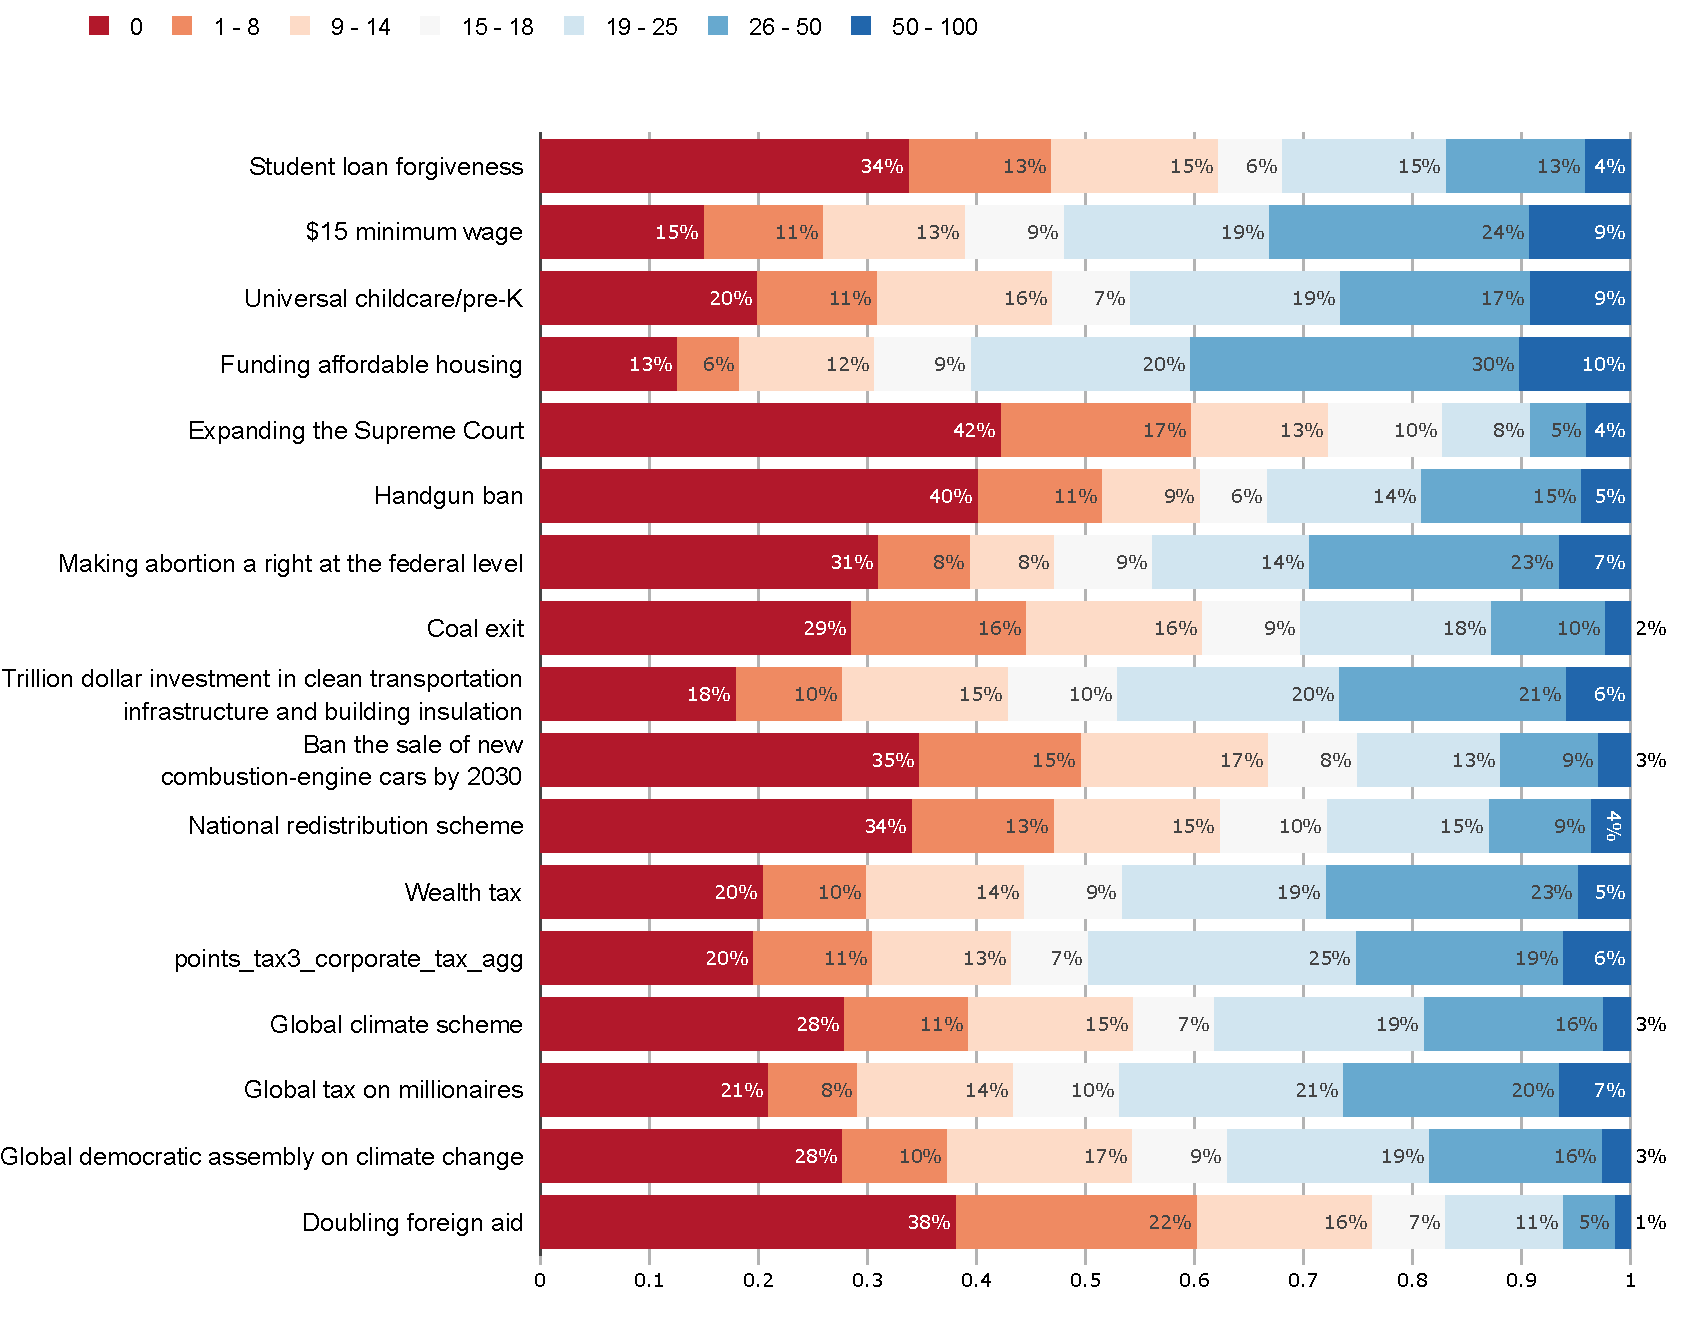
\includegraphics[width=\textwidth]{../figures/US1/points_us.pdf}} 
\end{figure}

% \begin{figure}[h!]
%     \caption{label}\label{fig:share_policies_supported}
%     \makebox[\textwidth][c]{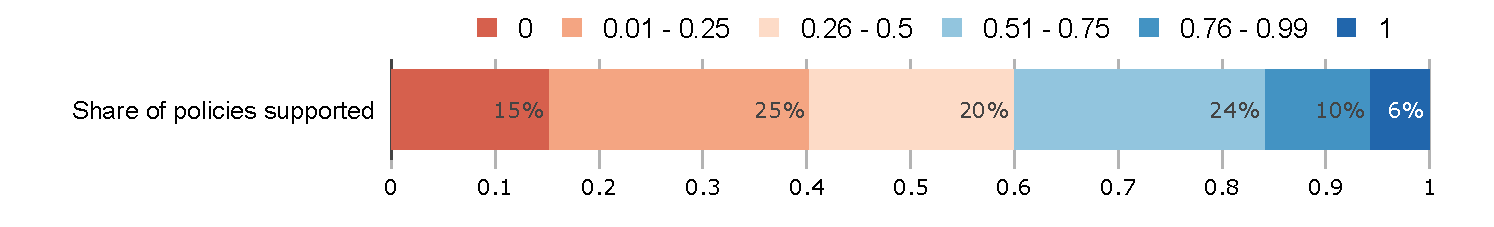
\includegraphics[width=\textwidth]{../figures/US1/share_policies_supported.pdf}} 
% \end{figure} % TODO? uncomment?

% \begin{figure}[h!]
%     \caption{label}\label{fig:vars}
%     \makebox[\textwidth][c]{\includegraphics[width=\textwidth]{../figures/US1/vars.pdf}} 
% \end{figure}
